% Drawing 81/03-6 -- folder 81, batch 03, archive page 53 (PDF page 54).
% Transcription: en tête à gauche, un croquis au crayon repassé à l'encre : deux lobes accolés, marqués « bi » et « bi », joints par un trait vertical épais dont les extrémités portent chacune une flèche courbe.
% Kind: two lobes glued along an edge (bi, bi). Method 2 (schematic redraw from the facsimile). Status: partial.
% Notes: Two lobes in pencil, side by side, each marked « bi », meeting at a narrow waist; in ink, a heavy vertical stroke across the waist, with at its top a short curved arrow (concave upwards, head at the right) and at its foot a short curved arrow (head at the left). The vertical stroke is drawn between the middles of the two arrows. Left out: the pencil doublings of the right lobe and the faint stroke that runs on from the foot of the waist to the lower right. Still differs: the lobes are smooth curves through points read on his outlines; the two curved arrows are schematic. Redrawn 2026-11-10 (issue 128): to check again.
% Coordinates: 1 unit = 1 mm = 1/100 of the crop width (bbox in page fractions: [0.11, 0.08, 0.42, 0.2]).
% Redrawn by Claude (claude-fable-5-2), issue #128, 2026-11-10; not checked by a human; not compiled (no TeX in the session).
% Rights: reproduces part of the work -- behind RENDER_TRANSCRIPTS, never published by itself.
\documentclass[tikz,border=3pt]{standalone}
\usepackage{amsmath,amssymb}
\usetikzlibrary{patterns,arrows.meta}
\tikzset{pencil/.style={black!45}, struck/.style={black!35}, mpt/.style={circle,draw,inner sep=1.3pt}, pt/.style={circle,fill,inner sep=0.9pt}, opt/.style={circle,draw,fill=white,inner sep=1.1pt}}
\begin{document}
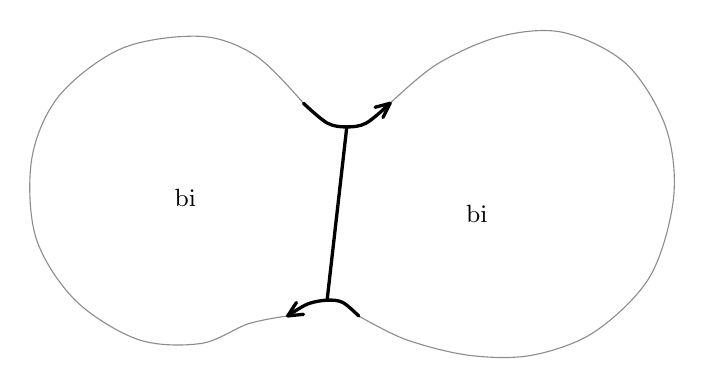
\begin{tikzpicture}[x=1mm,y=1mm,line cap=round,line join=round,font=\scriptsize]
\draw[pencil] plot[smooth, tension=0.55] coordinates {(43,-19) (37,-13) (30,-10.5) (20,-12) (12,-18) (8.5,-26) (9,-36) (14,-44) (22,-49) (30,-49.5) (36,-47) (41,-46)};
\draw[pencil] plot[smooth, tension=0.55] coordinates {(54,-19) (60,-14) (68,-10.5) (76,-10) (84,-14) (89,-22) (90,-31) (87,-41) (80,-48) (72,-51) (64,-51) (56,-49) (50,-46)};
\draw[very thick] plot[smooth, tension=0.55] coordinates {(43,-19) (46,-21.5) (48.5,-22) (51,-21.5) (54,-19)};
\draw[very thick] (52.1,-19.5) -- (54,-19) -- (53.1,-20.8);
\draw[very thick] (48.5,-22) -- (46,-44);
\draw[very thick] plot[smooth, tension=0.55] coordinates {(50,-46) (48,-44.3) (46,-44) (43.5,-44.5) (41,-46)};
\draw[very thick] (43,-45.8) -- (41,-46) -- (42.1,-44.3);
\node[inner sep=1pt] at (28,-31) {\small bi};
\node[inner sep=1pt] at (65,-33) {\small bi};
\end{tikzpicture}
\end{document}
